Let 
\begin{align}
    \vec{A}= \myvec{x\\-1} , \vec{B} = \myvec{2\\1} , \vec{C} = \myvec{4\\5}
\end{align}

Now,
\begin{align}
    \vec{B}-\vec{A} & = \myvec{2-x\\1-(-1)}\\
                    & = \myvec{2-x\\2}
\end{align}
\begin{align}
    \vec{B}-\vec{C} & = \myvec{2-4\\1-5}\\
                    & = \myvec{-2\\-4}
\end{align}

Forming the matrix $\vec{M}$,
\begin{align}
    \vec{M} & = \myvec{\vec{B}-\vec{A}  &  \vec{B}-\vec{C}}^\top \\
            & =\myvec{2-x & 2\\2 & -4}^\top\\
            & = \myvec{2-x & 2 \\ -2 & -4}
\end{align}

Using matrix transformation,


\begin{align}
 \vec{M} = \myvec{2-x & 2\\-2 & -4}
 \xleftrightarrow{\text{$R_2$}\rightarrow{\text{$R_2/2$}}} 
 \myvec{2-x & 2 \\-1 & -2}\\
 \xleftrightarrow{\text{$R_2$}\rightarrow{\text{$R_2 + R_1$}}}
 \myvec{2-x & 2 \\1-x & 0}
\end{align}
\begin{align}
 rank(\vec{M}) = 1 &\implies  R_2 =0 \\
 \text{or, }
            x=1
\end{align}
See Fig.          \ref{aug/2/9/plot}.
\begin{figure}[!h]
         \centering
         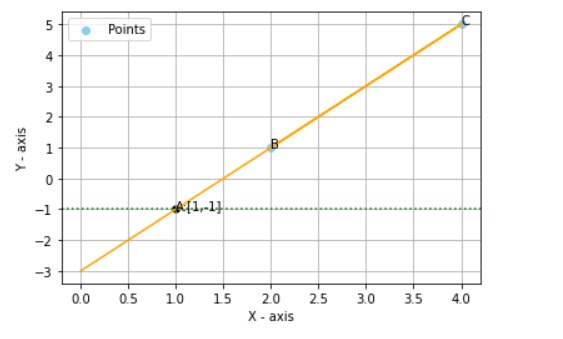
\includegraphics[width=\columnwidth]{solutions/aug/2/9/figures/figure.jpeg}
         \caption{Plot of the line }
         \label{aug/2/9/plot}
\end{figure}



